%%%%%%%%%%%%%%%%%%%%%%%%%%%%%%%%%%%%%%%%%%%%%%%%%%%%%%%%%%%%%%%%%%%%%%%%%%%%%%%%
%% Plantilla de memoria en LaTeX para la ETSIT - Universidad Rey Juan Carlos
%%
%% Por Gregorio Robles <grex arroba gsyc.urjc.es>
%%     Grupo de Sistemas y Comunicaciones
%%     Escuela Técnica Superior de Ingenieros de Telecomunicación
%%     Universidad Rey Juan Carlos
%% (muchas ideas tomadas de Internet, colegas del GSyC, antiguos alumnos...
%%  etc. Muchas gracias a todos)
%%
%% La última versión de esta plantilla está siempre disponible en:
%%     https://github.com/gregoriorobles/plantilla-memoria
%%
%% Para obtener PDF, ejecuta en la shell:
%%   make
%% (las imágenes deben ir en PNG o JPG)

%%%%%%%%%%%%%%%%%%%%%%%%%%%%%%%%%%%%%%%%%%%%%%%%%%%%%%%%%%%%%%%%%%%%%%%%%%%%%%%%

\documentclass[a4paper, 12pt]{book}
%\usepackage[T1]{fontenc}

\usepackage[a4paper, left=2.5cm, right=2.5cm, top=3cm, bottom=3cm]{geometry}
\usepackage{times}
\usepackage[utf8]{inputenc}
\usepackage[spanish]{babel} % Comenta esta línea si tu memoria es en inglés
\usepackage{url}
%\usepackage[dvipdfm]{graphicx}
\usepackage{graphicx}
\usepackage{subfigure} 
\usepackage{float}  %% H para posicionar figuras
\usepackage[nottoc, notlot, notlof, notindex]{tocbibind} %% Opciones de índice
\usepackage{latexsym}  %% Logo LaTeX
\usepackage{listings}
\usepackage{color}
\usepackage{alltt}
\usepackage{fancyvrb}
\usepackage{minted}
\usepackage{hyperref}
\usepackage{multicol}

\title{Memoria del Proyecto}
\author{Nombre del autor}

\renewcommand{\baselinestretch}{1.5}  %% Interlineado

\begin{document}

\renewcommand{\refname}{Bibliografía}  %% Renombrando
\renewcommand{\appendixname}{Apéndice}

%%%%%%%%%%%%%%%%%%%%%%%%%%%%%%%%%%%%%%%%%%%%%%%%%%%%%%%%%%%%%%%%%%%%%%%%%%%%%%%%
% PORTADA

\begin{titlepage}
\begin{center}
\begin{tabular}[c]{c c}
%\includegraphics[bb=0 0 194 352, scale=0.25]{logo} &
\includegraphics[scale=0.25]{img/logo_vect.png} &
\begin{tabular}[b]{l}
\Huge
\textsf{UNIVERSIDAD} \\
\Huge
\textsf{REY JUAN CARLOS} \\
\end{tabular}
\\
\end{tabular}

\vspace{3cm}

\Large
GRADO EN INGENIERÍA EN TECNOLOGÍAS DE TELECOMUNICACIÓN

\vspace{0.4cm}

\large
Curso Académico 2015/2016

\vspace{0.8cm}

Trabajo Fin de Grado

\vspace{2.5cm}

\LARGE
ANÁLISIS Y BÚSQUEDA DE \textit{IDIOMS} PROCEDENTES DE REPOSITORIOS ESCRITOS EN PYTHON

\vspace{4cm}

\large
Autor : José Javier Merchante Picazo \\
Tutor : Dr. Gregorio Robles
\end{center}
\end{titlepage}

\newpage
\mbox{}
\thispagestyle{empty} % para que no se numere esta pagina


%%%%%%%%%%%%%%%%%%%%%%%%%%%%%%%%%%%%%%%%%%%%%%%%%%%%%%%%%%%%%%%%%%%%%%%%%%%%%%%%
%%%% Para firmar
\clearpage
\pagenumbering{gobble}
\chapter*{}

\vspace{-4cm}
\begin{center}
\LARGE
\textbf{Proyecto Fin de Grado}

\vspace{1cm}
\large
ANÁLISIS Y BÚSQUEDA DE \textit{IDIOMS} PROCEDENTES DE REPOSITORIOS ESCRITOS EN PYTHON

\vspace{1cm}
\large
\textbf{Autor :} Jose Javier Merchante Picazo \\
\textbf{Tutor :} Dr. Gregorio Robles Martínez

\end{center}

\vspace{1cm}
La defensa del presente Proyecto Fin de Grado se realizó el día \qquad$\;\,$ de junio de 2016, siendo calificada por el siguiente tribunal:


\vspace{0.5cm}
\textbf{Presidente:}

\vspace{1.2cm}
\textbf{Secretario:}

\vspace{1.2cm}
\textbf{Vocal:}


\vspace{1.2cm}
y habiendo obtenido la siguiente calificación:

\vspace{1cm}
\textbf{Calificación:}


\vspace{1cm}
\begin{flushright}
Fuenlabrada, a \qquad$\;\,$ de junio de 2016
\end{flushright}

\setlength{\parskip}{2mm}
%%%%%%%%%%%%%%%%%%%%%%%%%%%%%%%%%%%%%%%%%%%%%%%%%%%%%%%%%%%%%%%%%%%%%%%%%%%%%%%%
%%%% Dedicatoria

\chapter*{}
\pagenumbering{Roman} % para comenzar la numeracion de paginas en numeros romanos
\begin{flushright}
\textit{Dedicado a \\
mis padres, mi hermana y mi pareja}
\end{flushright}

%%%%%%%%%%%%%%%%%%%%%%%%%%%%%%%%%%%%%%%%%%%%%%%%%%%%%%%%%%%%%%%%%%%%%%%%%%%%%%%%
%%%% Agradecimientos

\chapter*{Agradecimientos}
%\addcontentsline{toc}{chapter}{Agradecimientos} % si queremos que aparezca en el índice
\markboth{AGRADECIMIENTOS}{AGRADECIMIENTOS} % encabezado 

Con este trabajo se pone fin a una gran etapa en mi vida. Recuerdo momentos de incertidumbre, de máximo estrés, de olvidarme de todo lo que me rodeaba dedicándome exclusivamente a estudiar, no obstante siempre me compensó. Recuerdo esos grandes momentos de felicidad cuando en el Portal Servicios se reflejaba una buena nota, fruto del esfuerzo y disfrute en algunas asignaturas o algún aprobado que sabía a la máxima calificación.

Pero en todo este tiempo no he estado solo, he estado acompañado de grandes personas a las que no puedo dejar de agradecer su constante apoyo.

Agradezco a Gregorio Robles, mi tutor de este trabajo, por seleccionarme para la realización de una beca de colaboración con el departamento, por creer y confiar en mí. Por ayudarme y asesorarme durante, no solo este trabajo, sino también a nivel profesional.

Me gustaría agradecer también a mi familia, especialmente a mis padres y a mi hermana que siempre estuvieron preocupándose por mi, apoyándome y animándome a continuar cuando las cosas no salían todo lo bien que yo esperaba o alegrándose cuando alcanzaba mis metas.

También quisiera agradecer estos 4 años de carrera a mis compañeros que han estado junto a mi, sobre todo a Joel, al que conocí el primer día de llegar a la universidad, y que ha compartido conmigo esta larga etapa.

Por último, y no menos importante, agradecer a mi novia su paciencia por todos aquellos momentos de desesperación, por apoyarme cuando los resultados no eran los más deseados y estar dispuesta a ayudarme en todo lo que pudiera durante todo este tiempo.

A todos ellos, les debo este gran progreso en mi vida, ¡gracias!


%%%%%%%%%%%%%%%%%%%%%%%%%%%%%%%%%%%%%%%%%%%%%%%%%%%%%%%%%%%%%%%%%%%%%%%%%%%%%%%%
%%%% Resumen

\chapter*{Resumen}
%\addcontentsline{toc}{chapter}{Resumen} % si queremos que aparezca en el índice
\markboth{RESUMEN}{RESUMEN} % encabezado

El proyecto desarrollado trata sobre la creación de una herramienta especializada en la localización de elementos Python avanzados.

Además, obtiene una gran cantidad de repositorios almacenados en GitHub, escritos en este mismo lenguaje, para su posterior análisis con este programa y la explicación de las conclusiones alcanzadas.

El desarrollo de este proyecto se ha realizado con el lenguaje de programación Python, así como con otras librerías o herramientas como es el caso de \textit{pygments} para fragmentar el código, Pandas para realizar un análisis de una gran cantidad de datos o \textit{MongoDB} para almacenar los resultados obtenidos.

La realización de este proyecto ha requerido de un trabajo de investigación y documentación de las principales expresiones avanzadas del lenguaje empleado. Posteriormente se procedió a la recogida de datos y su correspondiente análisis, estudiando las resoluciones logradas.


%%%%%%%%%%%%%%%%%%%%%%%%%%%%%%%%%%%%%%%%%%%%%%%%%%%%%%%%%%%%%%%%%%%%%%%%%%%%%%%%
%%%% Resumen en inglés

\chapter*{Summary}
%\addcontentsline{toc}{chapter}{Summary} % si queremos que aparezca en el índice
\markboth{SUMMARY}{SUMMARY} % encabezado

The developed project is about the creation of a specialized tool, focus on locating Pythonic idioms from a big amount of repositories.

This project involves downloading a lot of repositories stored on GitHub, locating all the idioms, and making an analysis of the results in order to get some conclusions and explain them.

The development of this project has been completed with the use of Python programming language, as well as others libraries or tools such as the case of Pygments in order to obtain the tokens from the code, Pandas for analyzing all the idioms found, or MongoDB for storing the results in a database.

The realization of this project has required a research and documentation of the major advanced expressions of the language used. Then, we proceeded to collect all the data and make the analysis. 

%%%%%%%%%%%%%%%%%%%%%%%%%%%%%%%%%%%%%%%%%%%%%%%%%%%%%%%%%%%%%%%%%%%%%%%%%%%%%%%%
%%%%%%%%%%%%%%%%%%%%%%%%%%%%%%%%%%%%%%%%%%%%%%%%%%%%%%%%%%%%%%%%%%%%%%%%%%%%%%%%
% ÍNDICES %
%%%%%%%%%%%%%%%%%%%%%%%%%%%%%%%%%%%%%%%%%%%%%%%%%%%%%%%%%%%%%%%%%%%%%%%%%%%%%%%%

% Las buenas noticias es que los índices se generan automáticamente.
% Lo único que tienes que hacer es elegir cuáles quieren que se generen,
% y comentar/descomentar esa instrucción de LaTeX.

%%%% Índice de contenidos
\tableofcontents 
%%%% Índice de figuras
\cleardoublepage
%\addcontentsline{toc}{chapter}{Lista de figuras} % para que aparezca en el indice de contenidos
\listoffigures % indice de figuras
%%%% Índice de tablas
%\cleardoublepage
%\addcontentsline{toc}{chapter}{Lista de tablas} % para que aparezca en el indice de contenidos
%\listoftables % indice de tablas


%%%%%%%%%%%%%%%%%%%%%%%%%%%%%%%%%%%%%%%%%%%%%%%%%%%%%%%%%%%%%%%%%%%%%%%%%%%%%%%%
%%%%%%%%%%%%%%%%%%%%%%%%%%%%%%%%%%%%%%%%%%%%%%%%%%%%%%%%%%%%%%%%%%%%%%%%%%%%%%%%
% INTRODUCCIÓN %
%%%%%%%%%%%%%%%%%%%%%%%%%%%%%%%%%%%%%%%%%%%%%%%%%%%%%%%%%%%%%%%%%%%%%%%%%%%%%%%%

\cleardoublepage
\chapter{Introducción}
\label{sec:intro} % etiqueta para poder referenciar luego en el texto con ~\ref{sec:intro}
\pagenumbering{arabic} % para empezar la numeración de página con números

En este primer capítulo se abordará una visión genérica sobre los conceptos previos necesarios para entender el desarrollo de este proyecto. Se continuará con un pequeño epígrafe sobre las motivaciones que han propiciado la elaboración del mismo, así como se concluirá con una reseña a la estructura que sigue este trabajo.

\section{Conceptos previos}
Un lenguaje de programación permite a los programadores escribir una serie de instrucciones y algoritmos de una manera bastante simple en comparación al código máquina. De esta forma, permite simplificar de la realización de una determinada tarea en un ordenador, en la medida de lo posible, y la creación de nuevos programas.

La mayoría de lenguajes de programación tienden a seguir unos convenios, o unas guías de estilo como la tabulación, longitud de linea, convenios de nombre, etc., que en el caso de Python es PEP8, y se han diseñado herramientas para comprobarlo como PyFlakes, Pylint, PyChecker, etc.

Por otro lado, todos los lenguajes de programación tienen unos determinados \textit{idioms}, es decir, unas determinadas palabras o expresiones que son propias de cada lenguaje. Aprender dichos misterios de un lenguaje de programación junto a todas estas expresiones que se pueden encontrar, puede llevar años, que se adquieren al colaborar con programadores que tienen más experiencia, o leyendo código de libros avanzados como pueden ser “Pro Python” o “Python Cookbook”.

Para poner un ejemplo, una persona que tiene experiencia en C, la expresión
\begin{minted}{c}
    for (int i=0; i<list_length; i++){...}
\end{minted}
es un \textit{idiom} que suele usar habitualmente para iterar sobre un array, y sin embargo, no suelen utilizar otras estructuras para ello como \verb|do{...}while(...)|.
Aplicándolo al caso de Python, para iterar sobre una lista, siempre tiendes a usar \verb|for item in list| y a pesar de que no es la única forma que existe, es la más \textit{pythonic} consiguiendo un código más legible.

Muchos de los programadores que utilizan el lenguaje Python lo usan como si estuvieran programando en otro lenguaje, es decir, sin la utilización de dichos \textit{idioms}. Además, muchos de los programadores que empiezan a conocer este lenguaje, aprenden a partir de libros que no profundizan demasiado; es por ello que se hace necesario el desarrollo de una aplicación que ayude y facilite a éstos el conocimiento de nuevos elementos avanzados. 

Por siguiente, una de las principales finalidades de la realización de este programa, ha sido el estudio y la creación de una herramienta para que cualquier persona u organización, tanto con mucha experiencia como “junior”, pueda hacer un estudio de sus repositorios, aprendiendo qué elementos \textit{pythonic} aun no conoce, y sin embargo podrían serle de gran utilidad.

Por último, apuntar que mediante este programa se ha realizado un estudio de más de 70.000 repositorios gracias al software libre de GitHub, y se han obtenido resultados muy singulares que posteriormente analizaremos.



\section{Motivación}
Una de las grandes motivaciones que nos ha llevado a la realización de este Trabajo de Fin de Grado, ha sido el desarrollo de una aplicación para que todos los programadores, interesados en mejorar sus conocimientos de Python, puedan hacerlo de una manera sencilla, sin recurrir a los ``famosos libros pesados" de más de 400 hojas. Esta herramienta, supone una forma de ahorrar mucho tiempo y recursos económicos que tan valiosos son en nuestros días.

Actualmente, existe una gran cantidad de programadores que utilizan el lenguaje Python, y que dedican gran parte de su tiempo y esfuerzo a realizar tareas simples de manera compleja. Con la ayuda de una nueva herramienta, todo esto podría simplificarse mediante el aprendizaje de nuevos modismos propios de este lenguaje. De esta forma, lo que antes se mostraba como complicado, ahora puede ser más accesible y sencillo.

Estas son algunas de las razones que nos han incentivado a la creación de esta nueva aplicación, cuyo fin último es la asistencia y ayuda a todas las personas que utilicen Python.

\section{Estructura de la memoria}
En esta sección se trata de detallar la estructura que se sigue a lo largo del proyecto para facilitar su orden y mejor comprensión para el lector.

\begin{itemize}
\item En la introducción ubicada en el capítulo I, se realiza una descripción general del proyecto definiendo algunos conceptos necesarios, mostrando una motivación para el desarrollo del mismo y finalizando con una breve explicación de su estructura.
\item En el capítulo II se encuentran los objetivos, generales y específicos, que se pretenden lograr con la ejecución de este trabajo.
\item Situado en el capítulo III, se localiza el estado del arte, es decir, las diferentes tecnologías aplicadas a lo largo de este proyecto para una correcta evolución del mismo.
\item A continuación, en el capitulo IV, se menciona el desarrollo y la implementación del trabajo, definiendo las principales etapas y bloques, que se han ido tratando durante éste.
\item Tras la explicación de lo anterior, se determinan, en el capítulo V, los resultados obtenidos con una lista de análisis realizados.
\item Por último, en el capítulo VI, se hace referencia a las conclusiones, en las cuales aparecen principalmente los objetivos alcanzados, posibles trabajos futuros y una breve valoración personal.
\end{itemize}

%%%%%%%%%%%%%%%%%%%%%%%%%%%%%%%%%%%%%%%%%%%%%%%%%%%%%%%%%%%%%%%%%%%%%%%%%%%%%%%%
%%%%%%%%%%%%%%%%%%%%%%%%%%%%%%%%%%%%%%%%%%%%%%%%%%%%%%%%%%%%%%%%%%%%%%%%%%%%%%%%
% OBJETIVOS %
%%%%%%%%%%%%%%%%%%%%%%%%%%%%%%%%%%%%%%%%%%%%%%%%%%%%%%%%%%%%%%%%%%%%%%%%%%%%%%%%

\cleardoublepage
\chapter{Objetivos}
\label{chap:objetivos}

En esta sección, se pretende recoger todos los objetivos que han motivado la realización y desarrollo de esta herramienta.

\section{Objetivo general}
El objetivo principal de este proyecto es crear una herramienta para poder analizar y extraer los \textit{idioms} que se utilizan en proyectos programados en Python. De esta forma, mediante este programa, podemos medir el nivel de cultura de un determinado programador de este lenguaje.

Además, esta aplicación está pensada para ayudar y facilitar el trabajo de los programadores y conocer más a fondo las particularidades de Python.

Así mismo, con esta herramienta se pretende dar respuesta principalmente a las siguientes cuestiones:
\begin{itemize}
\item ¿Qué elementos \textit{pythonic} aparecen en un determinado proyecto escrito en Python?
\item ¿Dónde se localizan dichos \textit{idioms} en el proyecto?
\item ¿Quién escribió cada uno de los \textit{idioms} que encontramos a lo largo de los repositorios?
\item Etc.
\end{itemize}

De este modo, dado un repositorio o una lista de éstos, se pretende poder descargar todo su contenido y realizar un análisis de los mismos obteniendo una serie de conclusiones.



\section{Objetivos específicos}
Como objetivos más concretos, y desglosando las etapas por las que atraviesa la realización de este proyecto, podemos señalar las siguientes metas recogidas a continuación:


\begin{itemize}

\item Obtener información sobre los elementos \textit{pythonic} más eruditos de este lenguaje de programación.

\item Descargar una gran cantidad de repositorios de GitHub, cuyo lenguaje de programación principal sea Python, y realizar una búsqueda de los \textit{idioms} con la herramienta que se ha desarrollado.

\item Almacenar los resultados de dicha búsqueda en una base de datos.

\item Realizar un análisis sobre los resultados obtenidos de la exploración de todos los repositorios y de este modo obtener unas estadísticas sobre ellos.

\end{itemize}

En conclusión, lo que se busca es la realización de un análisis completo y exhaustivo de la mayor cantidad posible de repositorios escritos en Python, y de este modo, poder obtener una serie de conclusiones.




%%%%%%%%%%%%%%%%%%%%%%%%%%%%%%%%%%%%%%%%%%%%%%%%%%%%%%%%%%%%%%%%%%%%%%%%%%%%%%%%
%%%%%%%%%%%%%%%%%%%%%%%%%%%%%%%%%%%%%%%%%%%%%%%%%%%%%%%%%%%%%%%%%%%%%%%%%%%%%%%%
% ESTADO DEL ARTE %
%%%%%%%%%%%%%%%%%%%%%%%%%%%%%%%%%%%%%%%%%%%%%%%%%%%%%%%%%%%%%%%%%%%%%%%%%%%%%%%%

\cleardoublepage
\chapter{Estado del arte}
En esta sección se mencionan las tecnologías utilizadas para el desarrollo del programa centrándose principalmente en Python debido a que es la base principal del proyecto.



%%%%%%%%%%%%%%%%%%%%%% PYTHON %%%%%%%%%%%%%%%%%%%%%%
\section{Python} 
\label{sec:seccion1}

Python es un lenguaje de programación desarrollado a finales de los 80 y principios de los 90 por Guido van Rossum, cuya versión 1.0 del código fue publicada en 1994. Fue creado inspirándose en el lenguaje de programación ABC con todas sus ventajas, pero evitando sus inconvenientes y con la necesidad de crear un lenguaje de scripting. A lo largo de estos años, Python ha estado desarrollándose, obteniéndose nuevas versiones Python 2 o Python 3, que introducen significantes mejoras. 

Python es un lenguaje de programación de alto nivel, es interpretado y además interactivo, lo que permite probar pequeños bloques de código antes de introducirlos finalmente en un programa sin la necesidad del usuario tener que compilarlo, pero con el inconveniente de que la ejecución se realiza algo más lenta frente a otros lenguajes que tienen la necesidad de ser compilados antes de su ejecución.

Python tiene datos fuertemente tipados, es decir, una determinada variable de un tipo específico no se puede usar como si fuera de otro distinto a no ser que se realice previamente una conversión. Por otro lado tiene un tipado dinámico, por lo que los tipos de las variables no se comprueban durante la compilación sino durante la ejecución.

Python además tiene la ventaja de que es multiparadigma, lo que permite a los programadores poder elegir el estilo más deseado para determinadas tareas. En este caso se permiten el imperativo, el orientado a objetos y el funcional.

Por otro lado, Python está equipado de una librería estándar que le permite trabajar con procesamiento de Strings, protocolos de internet, ingeniería de software, interfaces de sistemas operativos, etc., y además tiene una plataforma con más de 80.000 paquetes extra, desarrollados por la comunidad, en la que se puede encontrar toda la variedad de módulos para nuestros programas.

Si se pudiera destacar algo de Python por encima de todo, sería por su sencillez y su fácil lectura. Tiene una sintaxis que hace que su programación sea bastante más amigable y fácil de entender frente a otros lenguajes de programación. Debido a que es un lenguaje de alto nivel, permite realizar operaciones complejas en pocas líneas de código, lo que facilita el escribir programas en menos tiempo y poder dedicarle más tiempo al diseño y a la depuración del código.

Python tiene un intérprete que está disponible para todas las plataformas, a pesar de que en un primer momento fuera diseñado especialmente para UNIX. Dado que el lenguaje es interpretado, no es necesario que el usuario realice la compilación, sino que es en el momento de la ejecución cuando se traduce a código máquina.

Además si se necesita crear un nuevo módulo o función para integrarlo se puede realizar fácilmente con el lenguaje de programación C, así como enlazar alguna librería que únicamente se encuentre en formato binario.

Debido a ser software libre, existen diversas implementaciones de éste como se pueden destacar Cpython, Jython, PyPy, IronPython, etc.

Por último, resaltar sobre todo la filosofía de Python, The Zen of Python \cite{peters2010zen}, una guía de principios compuesto por 20 aforismos descritos por Tim Peters, de los cuales hay escritos 19 y se puede encontrar en todos los intérpretes de Python: \\
\begin{itshape}
Beautiful is better than ugly. \\
Explicit is better than implicit. \\
Simple is better than complex. \\
Complex is better than complicated. \\
Flat is better than nested. \\
Sparse is better than dense. \\
Readability counts. \\
Special cases aren't special enough to break the rules. \\
Although practicality beats purity. \\
Errors should never pass silently. \\
Unless explicitly silenced. \\
In the face of ambiguity, refuse the temptation to guess. \\
There should be one-- and preferably only one --obvious way to do it. \\
Although that way may not be obvious at first unless you're Dutch. \\
Now is better than never. \\
Although never is often better than *right* now. \\
If the implementation is hard to explain, it's a bad idea. \\
If the implementation is easy to explain, it may be a good idea. \\
Namespaces are one honking great idea -- let's do more of those!
\end{itshape}



%%%%%%%%%%%%%%%%%%%%%% GIT %%%%%%%%%%%%%%%%%%%%%%
\section{Git} 
\label{sec:seccion2}

Git\footnote{https://git-scm.com/doc} es un sistema de control de versiones que está libremente distribuido y es de código abierto. Fue diseñado por Linus Torvalds (el padre del \textit{kernel} Linux) en 2005, cuyos objetivos principales fueron la velocidad y un diseño sencillo.

Un control de versiones, como es el caso de Git, es un sistema que almacena la historia de los cambios que se han realizado sobre un determinado fichero, permitiéndote en cualquier momento volver a un estado anterior, recuperar información o simplemente obtener el autor de la línea y cuando la introdujo o modificó la misma.

Esto permite olvidarse de realizar \textit{backups} y almacenar el código con distintas versiones con cada cambio que se realizara sobre un proyecto, por si en un momento dado dejaba de funcionar la aplicación y no recordabas la modificación que realizaste para volver a un estado anterior. Con el control de versiones al realizar un \textit{commit} de cada cambio no es necesario preocuparse por si deja de funcionar el proyecto entero, debido a que siempre se podrá ir a una versión anterior, o ver los cambios que produjeron el fallo.

Además de lo detallado previamente, Git y la mayoría de control de versiones en general, ofrecen una gran cantidad de recursos y ventajas, como por ejemplo, permitir a los desarrolladores crear ramas, trabajar dos personas sobre un mismo documento o mantener los ficheros de manera distribuida.

Algunas de los términos más comunes en el control de versiones y en Git, dentro de la gran cantidad que existen, son los siguientes:
\begin{itemize}
    \item El conjunto de datos y cambios que se han realizado sobre los ficheros que pertenecen a un mismo proyecto, se almacenan en \textbf{repositorios} que normalmente se encuentra en un servidor.
    \item Usualmente cuando se quiere añadir una nueva funcionalidad a un proyecto, sin modificar el resultado final de un programa, se suele crear una nueva rama (\textit{\textbf{branch}}) y sobre ella se aplican los cambios que se deseen.
    \item Cuando los cambios realizados sobre la nueva rama se quieren llevar al programa final, se dice que se hace un \textbf{\textit{merge}} con la rama principal añadiendo todos estos nuevos cambios.
    \item Existe un comando para obtener los cambios que otros usuarios han realizado sobre un repositorio, como es el caso de \textbf{\textit{git pull}}, y otro comando para añadir tus nuevas modificaciones al servidor que es denominado \textit{\textbf{git push}}.
    \item Para obtener el nombre de la persona que ha modificado una linea en un determinado fichero de un repositorio, se utiliza el comando \textbf{\textit{git blame}}.
\end{itemize}



%%%%%%%%%%%%%%%%%%%%%% PYGMENTS %%%%%%%%%%%%%%%%%%%%%%
\section{Pygments} 
\label{sec:seccion3}
Pygments\footnote{http://pygments.org/} es un motor de resaltado de sintaxis escrito en Python que soporta más de 300 lenguajes distintos.

Su principal finalidad es remarcar aquellas palabras o expresiones que son usuales o reservadas de un determinado lenguaje de programación, como puede ser el caso de Python, lenguajes de marcado como HTML, de scripting como es el caso de Bash y de otros tipos de formato de texto. 

Ofrece una salida en otro formato, con la sintaxis ya remarcada, como puede ser HTML, LaTeX, SVG u otros, pudiendo destacar dichas expresiones con distintas fuentes de letra, colores o tamaños.

Pygments es ampliamente utilizado, y está siendo usado por grandes organizaciones como Wikipedia o BitBucket en sus aplicaciones web.


En este proyecto se ha utilizado Pygments debido a su potencia, rapidez y sencillez para dividir el código Python en \textit{tokens} y ofrecerlos identificados por el tipo que son cada uno, para su posterior análisis.



%%%%%%%%%%%%%%%%%%%%%% MONGO DB %%%%%%%%%%%%%%%%%%%%%%
\section{MongoDB}
\label{sec:seccion4}
MongoDB\footnote{https://www.mongodb.com/} es una base de datos NoSQL basada en documentos. Este servicio de base de datos comenzó en 2007, pero fueron dos años después cuando empezó a comercializarse y no fue hasta 2011 cuando ya se pudo utilizar en producción \cite{banker2011mongodb}. 

Además es una base de datos libre, de código abierto y que está ampliamente utilizada en la industria. Empresas como Expedia o Forbes que manejan millones de usuarios, tienen implementadas una base de datos MongoDB desarrollada en poco tiempo, debido a la sencillez para almacenar todos sus datos.

Este sistema de almacenamiento guarda la información en estructuras denominadas BSON que son documentos similares a JSON que almacenan en cada campo tipos de datos específicos, arrays, u otros documentos.

Todos los documentos que tienden a tener una misma estructura están a su vez organizados en colecciones, que al mismo tiempo se almacenan en la base de datos.

Su versatilidad, rendimiento, escalabilidad, multiplataforma y sencillez al estar los datos almacenados en documentos JSON, hacen de esta base de datos una buena arquitectura sobre la que  poder almacenar grandes cantidades de información, como las que se presentan en este proyecto, para posteriormente poder hacer un análisis completo.



%%%%%%%%%%%%%%%%%%%%%% PANDAS %%%%%%%%%%%%%%%%%%%%%%
\section{Pandas} 
\label{sec:seccion5}
Python es un lenguaje de programación de alto nivel que ofrece estructuras de datos genéricas. Para el análisis de las mismas, no incluye demasiadas herramientas. Por ese motivo, Wes McKinney comenzó a desarrollar la librería Pandas en 2008 \cite{mckinney2012python}.

Pandas\footnote{http://pandas.pydata.org/} es una librería de código abierto basada en Python. Ofrece estructuras de datos rápidas, flexibles y eficientes, diseñadas para la realización de análisis de datos. Para obtener un mayor rendimiento, algunas de las partes están escritas en C o CPython.

Para ello, proporciona estructuras de datos simples como \textit{Series}, un \textit{array} de una dimensión con etiquetas en sus ejes, y \textit{Dataframes}, una potente estructura de datos tabulada de tamaño variable con ambos ejes etiquetados. Estas estructuras, permiten realizar una gran cantidad de operaciones sobre los datos, pudiendo ejecutar análisis estadísticos, mostrar su contenido sobre una gráfica, manipular su información o incluso manejar datos perdidos.

Además, ofrece una gran cantidad de recursos, tanto para obtener como para guardar la información en CSV, Excel, bases de datos relacionales y no relacionales, HDF5 y JSON.

Pandas también trabaja con otros paquetes de Python para manejar los datos como es el caso de \textit{NumPy} o librerías como \textit{matplotlib} para representar los datos sobre una gráfica.

Por último, destacar, que el uso de Pandas suele utilizarse sobre la aplicación web \textit{Jupyter Notebook}, una interfaz que proporciona un desarrollo en el navegador, ejecutándose el código en el servidor, para una mejor visualización de los datos. En el navegador se pueden crear programas para la representación de gráficos interactivos, simulaciones y otros, que permiten una computación interactiva en la web.

\section{GitHub} 
\label{sec:seccion6}
GitHub\footnote{https://github.com/} es un servidor web, nacido en 2008, que almacena repositorios Git de software libre y que cuenta con más de 14 millones de usuarios. 

Git permite almacenar los cambios en local, pero para desarrollar código entre varios programadores se hace necesario el uso de un servidor. Esta plataforma web, facilita precisamente ese objetivo, el desarrollo colaborativo de software, además de proporcionar herramientas como es el caso de seguimiento de incidencias, interfaz gráfica para comparación de código, y muchas más.

GitHub es uno de los servidores para el almacenamiento de código más popular del mundo. Es por ello, que se usa como fuente de información con el fin de descargar todos los repositorios de interés para su posterior análisis en este proyecto.

Ofrece una API (\textit{Application Programming Interface}) para poder acceder a toda la información almacenada, tanto de los repositorios como de los usuarios, y permitir de este modo realizar análisis y estadísticas, así como poder hacer búsquedas específicas.

Para acceder a dicha información no es necesaria la autenticación por parte del desarrollador, pero de este modo está limitado el número de peticiones por hora a 60. En caso de hacer peticiones a la API estando autenticado mediante un \textit{token}, te permite aumentar dicho límite hasta 5.000, una cantidad razonable si se quiere mantener el servicio estable.

La realización de más peticiones por hora no es posible, por lo tanto hace de proyectos que necesitan obtener grandes cantidades de información a partir de GitHub un proceso lento, tedioso y que dificulta en gran medida.


\section{GHTorrent} 
\label{sec:seccion7}
Son precisamente las dificultades mencionadas previamente en GitHub, las que hicieron necesaria la creación de una herramienta que solventara todos estos inconvenientes.

De esta forma, GHTorrent\footnote{http://ghtorrent.org/} es un proyecto de software libre enfocado principalmente a trabajos similares a éste, es decir, obtener una gran cantidad de datos de GitHub pero evadiendo las restricciones de 5.000 peticiones por hora. 

Para tal fin, monitoriza toda la actividad de GitHub gracias a las \textit{API keys} que ofrecen los usuarios y mantiene más de 4TB de documentos JSON comprimidos en una base de datos MongoDB y más de 1.500 millones de filas en una base de datos MySQL \cite{Gousi13}.

Este proyecto soluciona con creces el límite estipulado por GitHub, y ayuda a satisfacer las necesidades de los desarrolladores a la vez que quita carga de trabajo a los servidores de GitHub.

%%%%%%%%%%%%%%%%%%%%%%%%%%%%%%%%%%%%%%%%%%%%%%%%%%%%%%%%%%%%%%%%%%%%%%%%%%%%%%%%
%%%%%%%%%%%%%%%%%%%%%%%%%%%%%%%%%%%%%%%%%%%%%%%%%%%%%%%%%%%%%%%%%%%%%%%%%%%%%%%%
% DISEÑO E IMPLEMENTACIÓN %
%%%%%%%%%%%%%%%%%%%%%%%%%%%%%%%%%%%%%%%%%%%%%%%%%%%%%%%%%%%%%%%%%%%%%%%%%%%%%%%%

\cleardoublepage
\chapter{Desarrollo e implementación}

En esta sección se detallará la metodología seguida para poder obtener los resultados del proyecto y su posterior exposición de análisis y representaciones.

\begin{figure}[h]
\centering
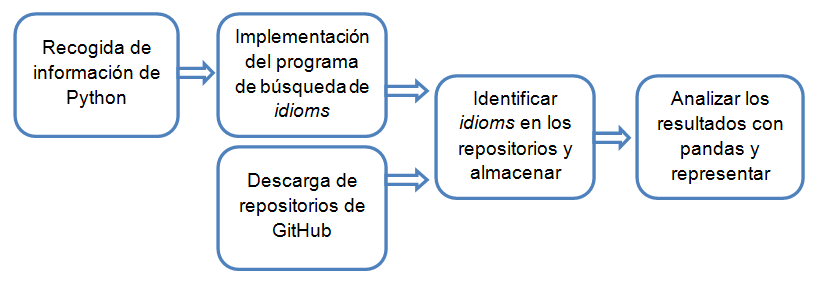
\includegraphics[width=160mm]{img/diagrama.png}
\caption{Diagrama del desarrollo}
\label{fig:diagrama}
\end{figure}

El desarrollo del proyecto, tal y como se indica en la figura \ref{fig:diagrama}, sigue diferentes etapas:
\begin{enumerate}
    \item Recogida de información e investigación sobre los elementos avanzados en Python.
    \item Análisis de cada fichero para obtener sus \textit{idioms} que supone uno de los pilares fundamentales del proyecto.
    \item Descarga de los repositorios cuyo principal lenguaje fuera Python. Esta etapa se ha realizado en paralelo a los epígrafes anteriores.
    \item Analizar todos los repositorios descargados para encontrar los elementos \textit{pythonic} que se consideran relevantes.
    \item Análisis de los resultados del punto anterior para la obtención de datos acerca de los repositorios escritos en Python.
\end{enumerate}

A continuación se procederá al análisis y desarrollo de cada una de las etapas mencionadas, especificando los detalles más significativos de este proyecto.

%%%%%%%%%%%%%%%%%%%%%%%%% RECOGIDA DE DATOS %%%%%%%%%%%%%%%%%%%%%%%%%%%
\section{Recogida de datos}  
\label{sec:recogida_de_datos}

Para empezar con el proyecto, la primera etapa, la más importante y a la que más tiempo tuvimos que dedicar, fue a documentarse de la gran cantidad de información que ofrece la comunidad de Python. En ésta, encontramos numerosos elementos, algunos muy sencillos de entender e identificar, y otros que a pesar de su complejidad, resultan singulares debido a las facilidades que ofrecen a la labor de programar una vez aprendidos.

La documentación la obtuvimos a partir de una gran variedad de libros, unos más sencillos y que ofrecían menos información sobre elementos \textit{pythonic} avanzados, como son el caso de \textit{Head First Python}, \textit{Introducing to Python} o \textit{Dive into Python}, otros que te mostraban la filosofía de Python a base de ejemplos simples como \textit{Effective Python} o \textit{Python Cookbook}, y otros en los que se focalizaban principalmente en explicar y exponer ejemplos de los elementos de Python más avanzados como son el caso de \textit{Pro Python} o \textit{Expert Python Programming}.

Además de la información obtenida a partir de los libros, también se han visualizado conferencias realizadas por personas más documentadas en Python y que han dedicado gran parte de su vida a ello, como puede ser el caso de Raymond Hettinger \cite{raymondhettinger}. En éstas se explican buenas prácticas para escribir un código más legible y elementos \textit{pythonic} que se suelen utilizar para determinadas circunstancias.

Así mismo, hemos centrado nuestra búsqueda en localizar más información en la web, hayando más documentación, aprendiendo, y perfeccionando más nuestro conocimiento en el lenguaje de Python.

A partir de toda esta información recogida, procedimos a la realización de una lista donde se detallaran algunos de los \textit{idioms} que deberían conocerse si se quisiera aprender Python y otros algo más avanzados que quizá utilizarían personas con un conocimiento más avanzado del lenguaje.

Por otro lado he incorporado una serie de \textit{anti-idioms} que tienden a utilizar programadores procedentes de otros lenguajes o que poseen poca experiencia para poder cerciorar su erróneo uso en algunas de las situaciones en las que aparecen.

Por su gran importancia y relevancia en este proyecto, hemos creído conveniente incluir una parte de esta extensa lista en el apéndice \ref{app:idioms}.
%%%%%%%%%%%%%%%%%%%%%%%%% OBTENCIÓN IDIOMS %%%%%%%%%%%%%%%%%%%%%%%%%%%
%\section{Implementación}  
%\label{sec:implementacion}
%%%%%%%%%% IDIOMS %%%%%%%%%%
\section{Obtención de \textit{idioms}}
\label{sec:obtencion_idioms}

La segunda parte del desarrollo del proyecto fue la estructuración del mismo, estudiando en primer lugar la manera de obtener un único \textit{idiom} a partir de un fichero.

Para tal fin, se usó la herramienta Pygments, un módulo escrito en Python para remarcar la sintaxis, pero cuya verdadera finalidad en este proyecto no ha sido exactamente esa. Hemos utilizado el motor que posee para que a partir de un cierto código, se obtenga cada palabra (\textit{token}) y de qué tipo es cada una de ellas. Para poner un simple ejemplo, a partir del siguiente fragmento de código:

\begin{minted}[]{python}
    for item in list:
        print item
\end{minted}

obtengo los \textit{tokens} de cada una de las palabras indicando el tipo al que pertenecen, como es el caso de \textit{(Token.Keyword, u'for')} o \textit{(Token.Operator.Word, 'in')}.

A partir de la sintaxis obtenida por Pygments, se tuvo que realizar una serie de funciones para el análisis de los ficheros, como por ejemplo, comprobar si los \textit{tokens} siguen una determinada secuencia, obtener los finales de línea o comparar con \textit{tokens} de referencia.

En consecuencia de todo lo explicado, la realización de un programa para obtener los \textit{idioms} de un determinado fichero a partir de su código sin la necesidad de importar ni ejecutar su contenido, estaba completada.

Durante el desarrollo de la obtención de los \textit{idioms} de un determinado fichero, se realizaron una serie de test que servirían para conocer si cualquier cambio que se realizara posteriormente sobre el código para optimizarlo, supondría un cambio significativo en el resultado de la ejecución y búsqueda de \textit{idioms}.

Para completar un poco más el análisis de los repositorios, parecía interesante obtener también el autor que había escrito cada linea, lo que haría de este proyecto algo más atractivo e interesante. Para tal fin, aprovechamos la salida que ofrece el comando \textit{git blame}. De esta forma y con la ayuda de simples expresiones regulares, a partir de la linea y el fichero donde se encontraba un \textit{idiom}, se podría obtener fácilmente el autor.

Una vez realizada la búsqueda y obtención de \textit{idioms}, se procedió a analizar repositorios enteros de código y la obtención del autor de las líneas donde se encontrara un \textit{idiom}.

Para concluir con un análisis más avanzado, nos dispusimos a analizar la mayor cantidad de repositorios que fuéramos capaces con los recursos disponibles, para su posterior estudio que comentaremos más adelante.




%%%%%%%%%% RECOGIDA DE DATOS %%%%%%%%%%
\section{Descarga de repositorios}
\label{sec:download_repositories}

El primer objetivo para la realización del análisis, fue obtener todos los repositorios de GitHub cuyo lenguaje de programación que predominara fuera Python, algo que según estuvimos comprobando, supondría una gran cantidad de información para realizar un buen estudio.

Debido a las restricciones de la API de GitHub, que limita a 5.000 peticiones autenticadas a la hora, supone una gran cantidad de tiempo identificar todos los repositorios escritos en Python y su posterior descarga. Por lo tanto, se optó por una vía más rápida recurriendo al uso de GHTorrent.

GHTorrent es un proyecto de software libre que permite obtener toda la información de los repositorios de GitHub evitando las restricciones de 5.000 peticiones por hora. Para ello nos descargamos la información que ofrecen de manera comprimida desde su web.

GHTorrent, además de bases de datos en MongoDB y MySQL, ofrece ficheros CSV, documentos en los cuales la información se muestra separada por comas que representarían las columnas de una tabla. Uno de esos ficheros mostraba información sobre los nombres de todos los repositorios en GitHub, su URL, el lenguaje principal, si era \textit{fork} de otro repositorio y algunos campos más, como por ejemplo, si había sido eliminado ya.

A partir de dicho fichero, se procedió al filtrado de toda la información que contenían, obteniendo únicamente, todos aquellos proyectos que estuvieran principalmente escritos en Python, que no fueran fruto de un \textit{fork} de otro repositorio y además, no hubieran sido eliminados ya.

La descarga de repositorios se realizó desde varias máquinas Linux. Mediante el comando \textit{git clone} se descargaban los repositorios y, a continuación, se almacenaban en un disco duro para su posterior análisis.

Las limitaciones que teníamos eran principalmente de espacio, puesto que únicamente disponíamos de algo más de 500GB de almacenamiento. Con dicha capacidad se consiguió descargar más de 70.000 repositorios escritos en Python, creando \textit{scripts} para eliminar todos aquellos ficheros que no fueran escritos en el lenguaje de programación objetivo, y conseguir con ello, más espacio. Dicha cantidad de repositorios suponemos que es una muestra bastante razonable para poder realizar análisis sobre ellos con unos resultados bastante precisos y significativos que pasaremos a analizar posteriormente.



%%%%%%%%%% obtencion de idioms a partir de los repositorios %%%%%%%%%%
\section{Obtención de \textit{idioms} a partir de los repositorios}
\label{sec:find_idioms_repos}

En esta sección se comentará el desarrollo del análisis de los repositorios para obtener los \textit{idioms} más significativos.

Para la localización de los \textit{idioms} dentro de los repositorios, se utilizó el programa descrito previamente en la sección \ref{sec:obtencion_idioms}, con el cual, llevando a cabo una búsqueda en los ficheros Python de los repositorios, se obtenían los elementos \textit{pythonic} más relevantes para la consecución de los objetivos.

Cuando comenzamos el análisis de los 70.000 repositorios, se tuvo que realizar un montaje de una base de datos MongoDB en la máquina local, para posteriormente almacenar todos los resultados que se obtuvieran, como consecuencia de hallar los \textit{idioms}.

Los resultados de cada repositorio se almacenaron en documentos independientes. Cada uno de éstos está compuesto por el nombre del \textit{idiom} que se encuentra en el repositorio y una lista indicando el fichero donde se localiza, el número de linea, el nombre del autor y otra información como el nombre del método encontrado en el caso de los \textit{magic methods}.

Debido a que el fichero creado únicamente localizaba los \textit{idioms} dentro de un fichero, se realizó un segundo programa que importaba a éste como un módulo y se utilizaban sus funciones.

En este nuevo fichero Python se hacía necesaria la creación de funciones para localizar únicamente los ficheros que fueran Python para analizarlos. Por otro lado, se utilizó el módulo PyMongo para conectar con la base de datos MongoDB y facilitar las operaciones.

En esta sección, se encontraron algunos \textit{bugs} del programa principal que fueron resueltos satisfactoriamente en la medida de lo posible. Algunos de los repositorios, no excesivos, contenían un fichero que provocaban una ralentización del análisis debido a su tamaño, pero que en su interior no contenían código Python o elementos que fueran objeto de búsqueda, a pesar de contener la terminación \textit{.py}. Para evitar estos ficheros, se procedió a la realización de un temporizador para detener el análisis de un fichero si se prolongaba de manera excesiva.



%%%%%%%%%% analyze idioms %%%%%%%%%%
\section{Análisis de los \textit{idioms} obtenidos}
\label{sec:analyze_idioms}

Una vez terminó de realizarse la obtención de \textit{idioms}, un proceso lento sabiendo que son más de 500 GB de datos, se procedió al análisis de los mismos con la librería Pandas.

Pandas es un paquete permite el estudio de grandes cantidades de datos, facilitando a Python al manejo de los mismos con estructuras mejor optimizadas para mejorar el rendimiento.

Los datos de la búsqueda, que permanecían almacenados en una base de datos MongoDB, suponían una gran cantidad de información para cargarla y manejarla de manera dinámica, por lo tanto, se hizo necesaria una conversión previa de los datos y obtener, de este modo, un fichero CSV.

El hecho de pasar la información de la base de datos a este tipo de formato, supondría ocupar un mayor tamaño, pero permitiría cargarlo con mayor rapidez sobre Pandas, debido a que éste módulo ofrece muchas más facilidades para obtener los datos en este tipo de formato, y por lo tanto, se mejoraría el rendimiento que es más importante frente a la cantidad de memoria usada hoy en día.

Con la ayuda de Pandas, se ha logrado analizar toda la información para la extracción de algunas estadísticas, así como conclusiones para una posterior mejora del programa.

Las conclusiones extraídas se mencionarán en el próximo capítulo, se han realizado análisis de los datos para obtener, por indicar un ejemplo, los \textit{idioms} más utilizados, la cantidad de \textit{idioms} encontradas en cada repositorio, así como unos estudios de la localización de los elementos \textit{pythonic} dentro de los ficheros.

%%%%%%%%%%%%%%%%%%%%%%%%%%%%%%%%%%%%%%%%%%%%%%%%%%%%%%%%%%%%%%%%%%%%%%%%%%%%%%%%
%%%%%%%%%%%%%%%%%%%%%%%%%%%%%%%%%%%%%%%%%%%%%%%%%%%%%%%%%%%%%%%%%%%%%%%%%%%%%%%%
% RESULTADOS %
%%%%%%%%%%%%%%%%%%%%%%%%%%%%%%%%%%%%%%%%%%%%%%%%%%%%%%%%%%%%%%%%%%%%%%%%%%%%%%%%

\cleardoublepage
\chapter{Resultados}
\label{chap:results}

Tras la búsqueda de los \textit{idioms}, y la identificación de más de 22.000.000 de \textit{idioms} localizados en más de 70.000 repositorios procedentes de usuarios de GitHub, se ha realizado un extenso análisis sobre todo ellos, obteniendo unos resultados entre los que cabe destacar los mencionados a continuación.



%%%%%%%%%%%%%%%%%%%%%%%%%%%%%%%%%%%%%%%%%%%%%%%%%%%%%%%%%%%%%%%%%%%%%%%%%%%%%%%%%%%%

\section{\textit{Idioms} más utilizados}
\label{sec:idioms_ranking}
Uno de los primeros análisis que se llevó a cabo fue la búsqueda de los elementos \textit{pythonic} más comunes, obteniendo lo mostrado en la figura \ref{fig:idiom_rank}.a.

\begin{figure}[t]
\centering
\subfigure[\textit{Idioms} más usados]{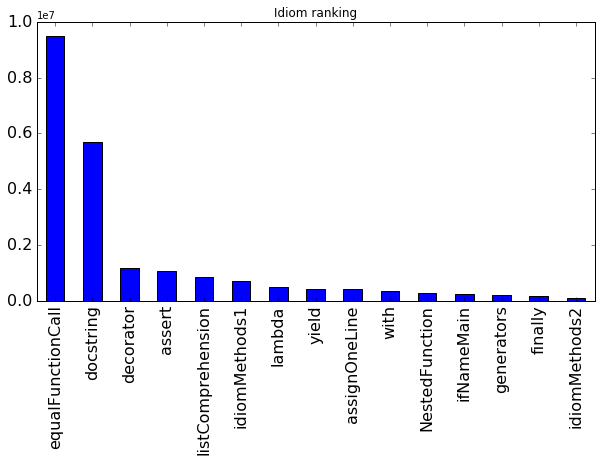
\includegraphics[width=79mm]{img/graphs/idiom_ranking.png}}
\subfigure[\textit{Idioms} más usados a partir del 3º]{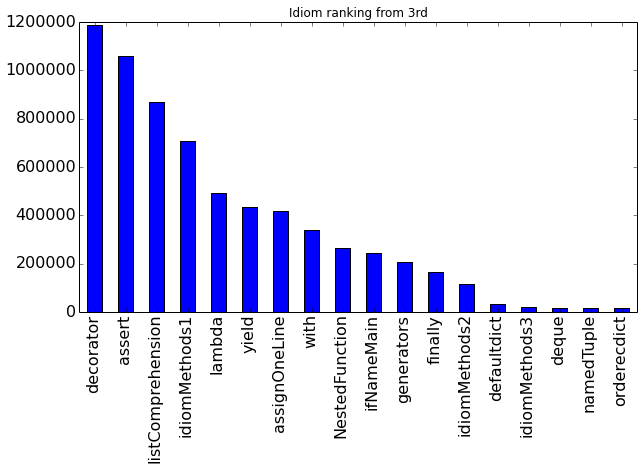
\includegraphics[width=79mm]{img/graphs/idiom_ranking_2.png}}
\caption{\textit{Idioms} más usados}
\label{fig:idiom_rank}
\end{figure}

Tal y como puede observarse, el primer \textit{idiom} procedente del análisis realizado previamente, es el de llamadas a una función con el operador igual entre sus argumentos, quizá, viendo esta gráfica, no es un \textit{idiom} para determinar si una persona conoce los elementos más avanzados de Python. Según se ha estado observando, gran cantidad de estos \textit{idioms} se encuentran en la misma línea al llamar a la misma función, y filtrando todos estos, la cantidad de esta categoría descendería a algo más de 7 millones de veces, manteniéndose en primera posición.

En segundo lugar, se encuentra la documentación, que más que ser un \textit{idiom}, puede ser de utilidad para la creación de estadísticas sobre la cantidad de repositorios y módulos que están documentados, una buena práctica en la programación. La mayor cantidad de repositorios, exactamente en torno al 75\% a partir de la muestra obtenida, se encuentran documentados. De esta misma forma, de todos los ficheros analizados, más del 65\% presentan documentación o comentarios en su contenido.

Los siguientes \textit{idioms}, que son los que quizá supongan un mayor interés, están representados en la figura \ref{fig:idiom_rank}.b.

Los \textit{decorators} son los \textit{idioms} que más se utilizan de la lista. Este tipo de \textit{idioms} permite la llamada a determinados métodos antes o después de la ejecución de una determinada función. Es posible que este elemento avanzado de Python haya sido seleccionado por gran cantidad de usuarios debido a su sencillez al utilizarlos y, de este modo, evitar repetir código.

A continuación se muestran otros como es el caso de \textit{assert}, una palabra reservada que permite encontrar \textit{bugs} o errores de una manera rápida y sencilla facilitando de esta forma la labor de depuración.

Otro de los \textit{idioms} que se usa con una gran frecuencia son las \textit{list comprehensions}. Permiten crear listas de una manera concisa lo que atrae a gran cantidad de programadores a usarlas.

En cuanto a los denominados \textit{magic methods}, que pasaremos a estudiar más adelante, cabe mencionar que se usan dentro de clases para poder aplicar determinadas funciones a las instancias de los objetos, un elemento de gran utilidad en numerosas ocasiones y es por ello que es ampliamente usado.



%%%%%%%%%%%%%%%%%%%%%%%%%%%%%%%%%%%%%%%%%%%%%%%%%%%%%%%%%%%%%%%%%%%%%%%%%%%%%%%%%%%%

\section{Porcentaje de aparición de \textit{idioms}}

No todos los \textit{idioms} aparecen en cada repositorio al menos una vez, debido a que no todos ellos han sido de utilidad para la realización de un proyecto, o quizá, los programadores que han escrito el código no saben de su existencia o quizá de su uso. Es por ello que se hace necesario una realización de unas estadísticas de la cantidad de repositorios en los que aparecen los elementos buscados.

En la figura \ref{fig:percentage_repos}, se muestra para cada uno de los \textit{idioms} el porcentaje de repositorios en los que aparecen a partir de la muestra obtenida procedente de GitHub.

\begin{figure}[!b]
\centering
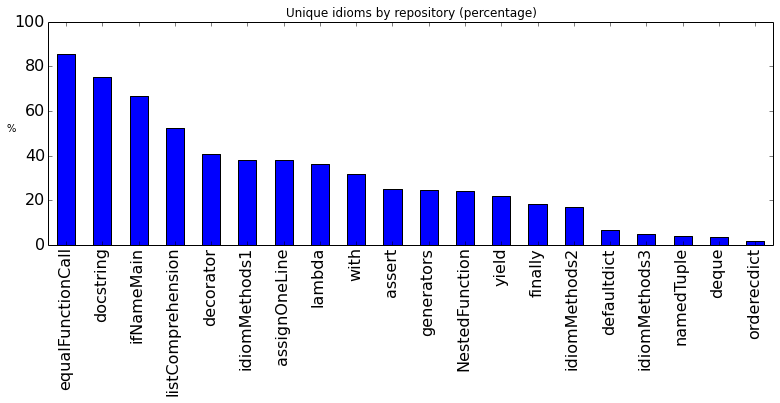
\includegraphics[width=140mm]{img/graphs/percentage.png}
\caption{Porcentaje de aparición en los repositorios}
\label{fig:percentage_repos}
\end{figure}

Cabe mencionar que el más utilizado es el de llamar a funciones con el operador igual. Se encuentra en el 85'4\% de los repositorios siendo el más utilizado quizá por su facilidad, por ejemplo, para llamar a una función cuyos argumentos no son necesarios al estar predefinidos, pero poder dar un nuevo valor a uno de ellos.

Remarcar que documentar los módulos y funciones en Python destaca, tal y como he mencionado previamente, en el 74'44\% de los repositorios.

Por otro lado, muchos de los repositorios contienen \verb|if __name__ == "__main__"| en al menos uno de sus ficheros el 66'65\% de las veces. Esta expresión, permite ejecutar la parte de código que contiene en su interior únicamente si se ejecuta directamente el módulo sin ser importado. Esto facilita la creación de ficheros en Python que sean módulos reusables además de programas independientes.

En cuanto a las \textit{list comprehensions}, breves sentencias que facilitan la creación de listas de una manera rápida, se encuentran en más del 50\% de los repositorios. De este modo se observa, que es un \textit{idiom} de gran utilidad en la programación en Python, y que se usa en una gran cantidad de repositorios.

Por último, destacar otros elementos \textit{pythonic} como son los \textit{decoratos}, los \textit{magic methods}, o palabras reservadas en Python como son el caso de \textit{lambda} o \textit{with}. Estos \textit{idioms} se encuentran entre el 30\% y 40\% de todos los repositorios analizados, y aunque no sea en más de la mitad, supone en muchos casos simplificar determinadas tareas.



%%%%%%%%%%%%%%%%%%%%%%%%%%%%%%%%%%%%%%%%%%%%%%%%%%%%%%%%%%%%%%%%%%%%%%%%%%%%%%%%%%%%

\section{Localización de los \textit{idioms}}

Otro de los análisis realizados sobre la obtención de elementos \textit{pythonic} ha sido la localización de los \textit{idioms} indicando en qué número de línea se han encontrado y observar, de este modo, si existe alguna peculiaridad a la hora de escribir el código.

Según se muestra en la figura \ref{fig:lines_idioms}.a, una gran cantidad de los \textit{idioms} se encuentran en la línea 1, a continuación disminuye de manera considerable y entre las líneas 10 a 50 vuelve a haber una gran cantidad, decreciendo posteriormente de manera exponencial. 

\begin{figure}[b]
\centering
\subfigure[\textit{Idioms} encontrados por número de línea]{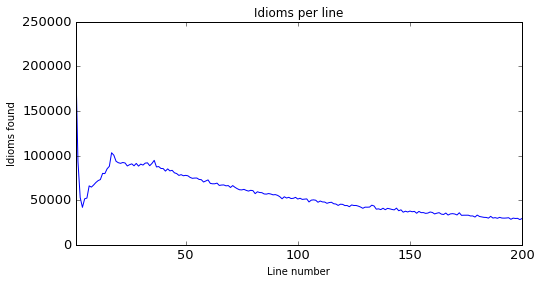
\includegraphics[width=99mm]{img/graphs/idioms_line.png}}
\subfigure[\textit{Idioms} en las primeras 10 líneas]{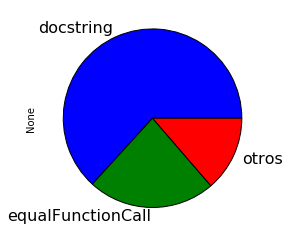
\includegraphics[width=59mm]{img/graphs/first_10_lines.png}}
\caption{Aparición de \textit{idioms} por cada línea}
\label{fig:lines_idioms}
\end{figure}

Dado que esta curva resulta singular, sobre todo en las primeras líneas, cuando pasamos a analizar los \textit{idioms} antes de la línea 10, tal y como se puede comprobar en la figura \ref{fig:lines_idioms}.b, se puede determinar que esa bajada es debida a que la mayoría de ficheros y módulos tienen unas líneas de documentación al comienzo, además de las importaciones que usualmente se realizan en esa zona. Esto conlleva a que las línea de código y los \textit{idioms} encontrados, no puedan aparecer en esas líneas, y en consecuencia, se muestren más adelante.

Tras analizar la causa de la peculiaridad de la curva de esa primera zona, se observa que la cantidad de elementos encontrado posteriormente se mantiene constante, y a continuación, comienza a decrecer de forma exponencial. La causa de esto, es debido a que existe una mayor cantidad de ficheros cortos en extensión, lo que favorece a encontrar más \textit{idioms} en las primeras líneas.



%%%%%%%%%%%%%%%%%%%%%%%%%%%%%%%%%%%%%%%%%%%%%%%%%%%%%%%%%%%%%%%%%%%%%%%%%%%%%%%%%%%%

\section{\textit{Magic methods} más utilizados}

Otro de los estudios realizados sobre los resultados ha sido la clasificación de los \textit{magic methods} más utilizados a los largo de todos los repositorios.
Para el análisis de este tipo de elementos \textit{pythonic}, se han dividido en tres clases diferentes:
\begin{enumerate}
    \item En primer lugar aquellos que eran más comunes de usar, son más sencillos y que se encuentran con mayor frecuencia entre los repositorios.
    \item En segundo lugar aquellos que ofrecen una mayor nivel en cuanto a programación se refiere, debido a que hay que conocer más en profundidad el lenguaje para saber cuándo utilizarlos.
    \item Por último, aquellos métodos, que ofreciendo una mayor complejidad para ser entendidos, muestran un mayor nivel de programador en Python.
\end{enumerate}

\begin{figure}[t]
\centering
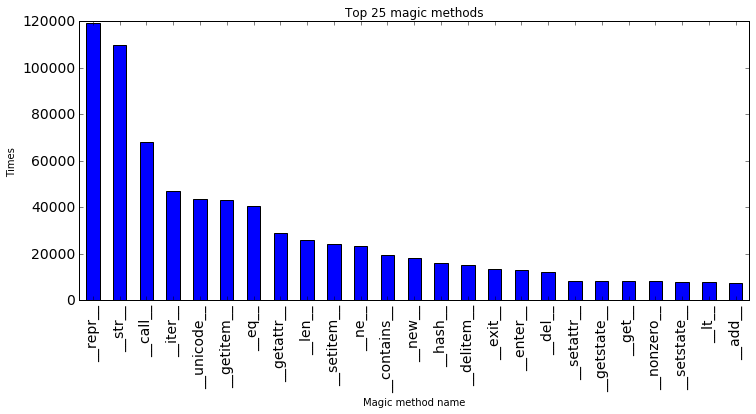
\includegraphics[width=140mm]{img/graphs/magic_methods.png}
\caption{25 \textit{magic methods} más utilizados}
\label{fig:magic_methods}
\end{figure}

Los resultados recogidos han sido los esperados. Según se ha podido mencionar previamente en la sección \ref{sec:idioms_ranking}, se han encontrado una mayor cantidad de métodos en la categoría que representa los \textit{idioms} más simples y comunes y una menor cantidad en la tercera categoría que corresponden a los que tienen una mayor complejidad.

La cantidad de métodos del primer grupo, supera lógicamente a los del segundo grupo, destacando, tal y como se muestra en la figura \ref{fig:magic_methods}, \textit{\_\_repr\_\_} y \textit{\_\_str\_\_}, debido a que son los que se usan en el momento de imprimir un objeto.

El siguiente más utilizado es \textit{\_\_call\_\_}, usado cuando se llama a la instancia de un objeto y el siguiente que destaca sobre el resto es \textit{\_\_iter\_\_}, utilizado para hacer un objeto iterable.

Por último, mencionar que hay algunos que suelen estar siempre juntos, como es el caso de \textit{\_\_enter\_\_} y \textit{\_\_exit\_\_}, que permiten implementar objetos que pueden ser usados fácilmente con la palabra reservada \textit{with}.

Del segundo grupo, destacan como los métodos más utilizados \textit{\_\_unicode\_\_}, un método utilizado cuando se llama a la función \textit{unicode()}, y que devuelve una cadena de caracteres como \textit{str()}, pero que en este caso es con formato \textit{unicode}. Otro método a destacar es \textit{\_\_hash\_\_}, que permite implementar el resultado de llamar a la función \textit{hash()} que devuelve un entero que se usa principalmente en comparación de las claves de un diccionario.

Por último, del tercer grupo destacar por ejemplo \textit{\_\_nonzero\_\_}, que define el comportamiento de la instancia de la clase cuando se llama a la función \textit{bool()} y tiene que devolver \textit{True} o \textit{False}.



%%%%%%%%%%%%%%%%%%%%%%%%%%%%%%%%%%%%%%%%%%%%%%%%%%%%%%%%%%%%%%%%%%%%%%%%%%%%%%%%%%%%

\section{Frecuencia de los \textit{idioms} analizados}
Los repositorios siguen una curva en la cantidad de \textit{idioms} que se utilizan dentro de ellos que tiene forma de una función exponencial.

\begin{figure}[t]
\centering
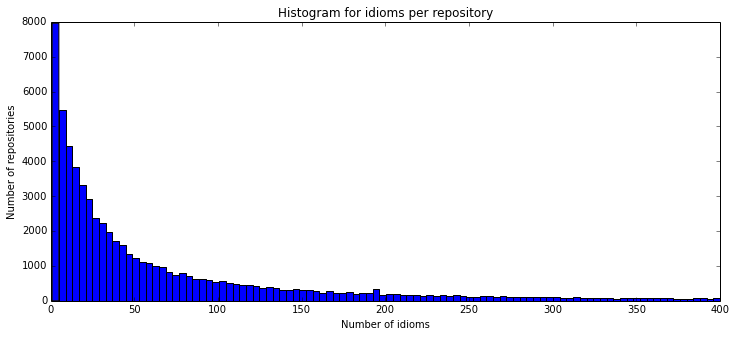
\includegraphics[width=140mm]{img/graphs/idioms_per_repository.png}
\caption{\textit{Idioms} por repositorio}
\label{fig:idiom_per_repo}
\end{figure}

Tal y como se puede observar en la figura \ref{fig:idiom_per_repo}, se puede concluir que la mayor parte de los repositorios tienden a tener pocos \textit{idioms} en sus repositorios, aunque no en todos ellos, debido a que más del 50\% de los repositorios tienen más de 40 \textit{idioms}. Una gran cantidad si se observa que muchos de ellos no tienen muchos ficheros en su interior.

Calculando la media de \textit{idioms} por repositorio es de 304'52, es decir, que se pueden observar una gran cantidad por cada repositorio. Si se omiten todos aquellos \textit{idioms} que se encuentran en la misma linea como es el caso de las llamadas a funciones con el operador igual, la media disminuye a 270'35, que se mantiene bastante alta.

Por otro lado, si se estudian la cantidad de \textit{idioms} que aparecen al menos una vez en cada repositorio, es decir, que no aparecen de manera duplicada en el mismo repositorio, podemos analizar la variedad de \textit{idioms} que se han utilizado en cada uno de éstos.

En esta parte del análisis, se observan resultados muy distintos a los anteriores observando la frecuencia, debido a que tal y como puede observarse en la figura \ref{fig:idioms_repos_abs}, la gran mayoría de los repositorios contienen en torno a 4 \textit{idioms} únicos, esto significa una muy pequeña cantidad.

Más del 50\% de los repositorios contienen 5 o menos elementos \textit{pythonic}, una muy pequeña cantidad sabiendo que se han buscado más de 120 diferentes, de los cuales, muchos de ellos están agrupados en \textit{magic methods}, pero desglosado para este estudio.

Por otro lado, sobre este último estudio, los repositorios contienen una media de 8'09 de \textit{idioms} únicos por repositorio, una cantidad realmente pequeña y que contrasta con los más de 250 mencionados anteriormente. Esto es principalmente debido, a que la mayoría de los \textit{idioms} utilizados en cada repositorio son poco variados y se repiten en multitud de ocasiones a lo largo de éstos.


\begin{figure}[t]
\centering
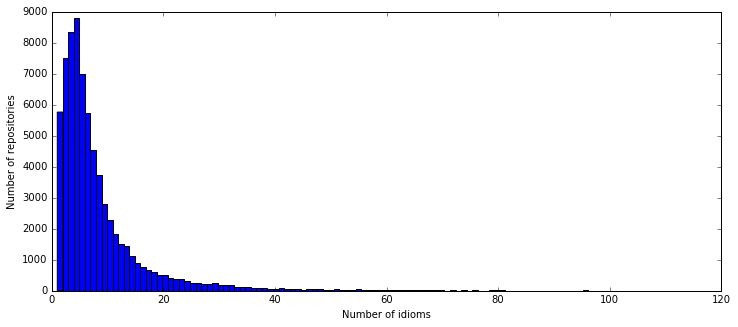
\includegraphics[width=140mm]{img/graphs/idioms_repos_abs.png}
\caption{Número de \textit{idioms} escritos en cada repositorio}
\label{fig:idioms_repos_abs}
\end{figure}



%%%%%%%%%%%%%%%%%%%%%%%%%%%%%%%%%%%%%%%%%%%%%%%%%%%%%%%%%%%%%%%%%%%%%%%%%%%%%%%%%%%%

\section{Análisis de los autores}

Por último, para conocer los datos acerca de los autores que escriben la gran cantidad de elementos \textit{pythonic} a lo largo de los repositorios, se ha realizado un estudio que muestra los resultados que se van a mencionar a continuación.

En primer lugar, hemos calculado el número de \textit{idioms} que utiliza cada autor de los repositorios analizados. Tal y como se puede observar en la figura \ref{fig:idiom_per_author}, la mayoría de los autores han escrito pocos \textit{idioms}, la causa de esto, puede ser debido a que no he analizado la totalidad de los repositorios en Python, y la mayoría de lo programadores seguro que tienen escrito más código.

\begin{figure}[t]
\centering
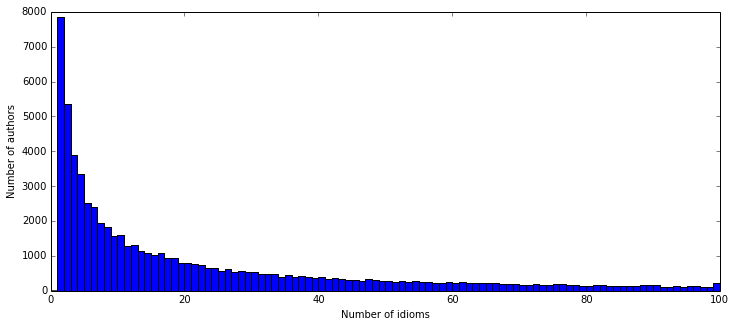
\includegraphics[width=140mm]{img/graphs/idioms_per_author.png}
\caption{\textit{Idioms} escritos por autor}
\label{fig:idiom_per_author}
\end{figure}

De los repositorios analizados, para realizar una pequeña estadística, puede decirse de media que han escrito 242'1, y si omitimos aquellos \textit{idioms} que aparecen duplicados en una misma línea, se obtiene que han escrito una media de 214'72, todo esto dependiente de la cantidad de repositorios que se han analizado de cada uno de los autores.

Por otro lado, he realizado un análisis de la cantidad de colaboradores que han aportado \textit{idioms} en cada proyecto. Uno de los proyectos que más variedad de autores tiene aportando \textit{idioms} es Pandas, tecnología que ha sido utilizada para la realización de este proyecto, que cuenta con 332 autores distintos. La gran mayoría de los repositorios presenta un único autor de los \textit{idioms} escritos o incluso dos, pero con 5 o más, tan solo se encuentran el 6\%.





%%%%%%%%%%%%%%%%%%%%%%%%%%%%%%%%%%%%%%%%%%%%%%%%%%%%%%%%%%%%%%%%%%%%%%%%%%%%%%%%
%%%%%%%%%%%%%%%%%%%%%%%%%%%%%%%%%%%%%%%%%%%%%%%%%%%%%%%%%%%%%%%%%%%%%%%%%%%%%%%%
% CONCLUSIONES %
%%%%%%%%%%%%%%%%%%%%%%%%%%%%%%%%%%%%%%%%%%%%%%%%%%%%%%%%%%%%%%%%%%%%%%%%%%%%%%%%

\cleardoublepage
\chapter{Conclusiones}
\label{chap:conclusiones}

En este capítulo se encuadran una serie de conclusiones y resultados obtenidos al final de la realización de este proyecto. Es necesario señalar que se han conseguido gran parte de los objetivos iniciales establecidos. Además, en este apartado se mencionan aquellas tecnologías aprendidas en materias cursadas a lo largo de la carrera, así como las que han sido de nuevo conocimiento. Por último, se mencionan posibles funcionalidades que mejorarían el proyecto y se concluirá con una valoración personal.

%%%%%%%%%%%%%%%%%%%%%%%%%%%%%%%%%%%%%%%%%%%%%%%%%%%%%%%%%%%%%%%%%%%%%%%%%%%%%%%%
\section{Consecución de objetivos}
\label{sec:consecucion-objetivos}

Como todo buen proyecto es necesario que tras la finalización del mismo, se hayan conseguido la mayor parte de las metas y logros esperados. Por todo ello, tras la realización y desarrollo de este trabajo es conveniente analizar, comprobar y valorar si se han conseguido o no los objetivos mencionados en el Capítulo 2.

Con la herramienta creada en este proyecto se ha logrado alcanzar el objetivo principal que persigue ayudar a todos los programadores en su trabajo con Python. Tras este proyecto, el buscar el número de elementos avanzados utilizados por éste ya es posible. Con este programa se puede identificar los \textit{idioms} empleados y aquellos, que en contraposición, no se han usado y quizá podrían haber sido utilizados. De esta manera, se permite al programador aprender nuevos \textit{idioms} y ampliar sus conocimientos en Python.

Así mismo, con esta aplicación el programador podrá dar respuesta a qué elementos \textit{pythonic} aparecen a largo de sus proyectos, ya que la aplicación identifica en su salida los que han aparecido. No obstante, esta herramienta no está libre de errores, y a pesar de que es bastante exacta, en ocasiones puede no dar el resultado deseado.

Además, con el programa desarrollado en este proyecto podemos localizar en qué linea y en qué fichero se encuentra ubicado un determinado \textit{idiom}. Esta labor permite analizar el código de otros programadores en búsqueda de elementos \textit{pythonic} y de este modo identificar su ubicación acortando el tiempo dedicado a ello.

Del mismo modo, a partir de la localización de los elementos \textit{pythonic} se puede obtener el autor que ha realizado la última modificación en la línea determinada previamente. Es por ello que no en todas las ocasiones es posible conocer al autor originario que escribió la línea objeto de estudio, pues si ésta ha sufrido diversas modificaciones, la identidad del mismo no se puede reconocer mediante este programa.

No podemos continuar este trabajo sin examinar también si se han alcanzado los objetivos específicos.

En este caso, dichos objetivos constituyen lo que ha sido la estructura y el desarrollo del trabajo, por lo tanto:

\begin{itemize}
\item Se ha logrado obtener información de los elementos más complejos gracias a un estudio exhaustivo de las distintas fuentes de información que estaban a nuestro alcance (libros, páginas web, conferencias...). De esta forma, hemos conseguido ampliar nuestros conocimientos, obtener nuevos y especializarnos en este lenguaje de programación.

\item Hemos conseguido descargar una muestra considerable de repositorios, más de 70.000, con la indispensable ayuda de la plataforma GHTorrent. Todo ello en un periodo de tiempo relativamente reducido, si tomamos de referencia la gran cantidad de almacenamiento ocupado. Además, hemos logrado que con la aplicación creada para este proyecto, se hayan localizado todos los \textit{idioms} existentes en cada repositorio.

\item En lo concerniente al almacenamiento de los elementos \textit{pythonic} encontrados, podemos determinar que este objetivo ha sido casi en su totalidad conseguido, puesto que en su mayoría se han almacenado sin ningún tipo de problema. No obstante, una parte de los repositorios no pudieron guardar sus resultados debido a que sobrepasaban el tamaño máximo por documento.

\item Por último, se ha alcanzado el objetivo de realizar un análisis y estadísticas sobre los \textit{idioms} encontrados. Esto se ha conseguido con la ayuda de Pandas que ha permitido representar gráficas y mostrar de una manera más sencilla los resultado obtenidos, facilitando así la labor de obtener conclusiones del estudio realizado.

\end{itemize}

En definitiva, prácticamente todos los objetivos propuestos al inicio de este proyecto, han sido abordados y superados con éxito.

%%%%%%%%%%%%%%%%%%%%%%%%%%%%%%%%%%%%%%%%%%%%%%%%%%%%%%%%%%%%%%%%%%%%%%%%%%%%%%%%
\section{Aplicación de lo aprendido}
\label{sec:aplicacion}

Han sido cuatro años de carrera los que me han hecho aprender numerosos conocimientos procedentes de diferentes áreas, quizá por ello, señalar una única asignatura que me haya aportado los conocimientos necesarios para la realización de este programa, no sería justo; puesto que pienso que ha sido un cúmulo de todas ellas con sus estudios, prácticas y demás trabajos los que creo que han forjado en mí una idea clara para la elaboración de este proyecto.

Quizá si tuviese que destacar algunas, serían las orientadas al área de la programación, puesto que su contenido y conocimientos se ajustan más al contexto de este trabajo. De esta forma mencionaría:

\begin{enumerate}
  \item Servicios de Aplicaciones Telemáticas (SAT) se trata de una asignatura que nos ha enseñado, entre otros conocimientos, las bases de la creación de servidores web con el lenguaje de programación Python. A consecuencia de ello, es evidente, que esta materia me ha aportado el entusiasmo y los conocimientos mínimos en Python para embarcarme en la iniciación de este proyecto.
  
  \item Fundamentos de la Programación (FDP) es la asignatura que proporciona la base fundamental del proyecto, la programación. Sin la ayuda de lo aprendido en esta asignatura, gran parte de lo desarrollado no podría haber sido abordado.
  
  \item Ingeniería de Sistemas de Información (ISI) se trata de una materia que a pesar de que la finalidad principal fuera la creación de un proyecto de un servidor y un cliente en grupos, me ha aportado los conocimientos necesarios para conocer la base de datos MongoDB y poder aplicarla a este proyecto. Además pude aprender en profundidad muchos de los comandos que Git ofrece.
\end{enumerate}

No puedo finalizar este epígrafe sin realizar una mención especial a todos mis profesores, que de una manera u otra, me han aportado todos sus conocimientos que estoy seguro que posteriormente aplicaré en mi carrera profesional.


%%%%%%%%%%%%%%%%%%%%%%%%%%%%%%%%%%%%%%%%%%%%%%%%%%%%%%%%%%%%%%%%%%%%%%%%%%%%%%%%
\section{Lecciones aprendidas}
\label{sec:lecciones_aprendidas}

A lo largo de este proyecto no sólo he podido poner en práctica los conocimientos aprendidos en el transcurso de la carrera, sino que este trabajo también me ha permitido adquirir nuevos conocimientos y experiencias acerca de, principalmente, tecnologías que antes estaban fuera de mi alcance.

De este modo quisiera destacar algunas de ellas que he adquirido durante el desarrollo y la realización de este trabajo:

\begin{enumerate}
  \item Python es un lenguaje de programación que comencé a conocer a partir de una asignatura mencionada previamente. En dicha materia, se obtienen conocimientos básicos acerca de su sintaxis, sin embargo, ha sido con el estudio proveniente de diversos recursos lo que ha originado el conocimiento de nuevos elementos avanzados.
  
  \item Otra de las tecnologías utilizadas que desconocía previamente, ha sido Pandas. Esta nueva librería me ha aportado un conocimiento general y básico para poder manejar grandes cantidades de datos de una manera sencilla y rápida.

  \item Pygments fue otra de las herramientas que nunca había utilizado e incluso desconocía de su existencia. Sin embargo, al tener que realizar una búsqueda de los \textit{idioms} tuve que documentarme y recurrir a él como fuente de este trabajo.
  
  \item Además, apliqué GHTorrent, un proyecto que me permitió la obtención de grandes cantidades de información acerca de los repositorios procedentes de GitHub. Esta tecnología captó mi atención ya que evitaba las restricciones que GitHub tenía, lo que facilitó mi labor en este proyecto.
  
  \item Por último, cabe mencionar el uso de la herramienta \LaTeX  que me ha permitido el desarrollo de esta memoria.
\end{enumerate}

Creo que es bastante importante la aplicación de todos estos conocimientos aprendidos, porque gracias a su utilización en este trabajo, me han permitido conocer de primera mano su funcionamiento y poder servirme de ellos en un futuro.


%%%%%%%%%%%%%%%%%%%%%%%%%%%%%%%%%%%%%%%%%%%%%%%%%%%%%%%%%%%%%%%%%%%%%%%%%%%%%%%%
\section{Trabajos futuros}
\label{sec:trabajos_futuros}

Es importante señalar que todo software necesita de una constante evolución, pues siempre existen utilidades aun no implementadas que pueden mejorar el programa desarrollado. Es por ello, que cabe mencionar este epígrafe en el que se abordarán posibles trabajos futuros a incorporar en el proyecto desarrollado. De esta forma, se podrá dotar a este programa de nuevas funcionalidades y optimizaciones de las ya existentes.

\begin{enumerate}
  
    \item Para completar un poco más el análisis, se podría incorporar la fecha y hora en la cual un determinado \textit{idiom} fue escrito por el autor del mismo. Así podríamos obtener una cronología y orden de los elementos \textit{pythonic} encontrados.
    
    
    \item Otra posible funcionalidad, sería facilitar la realización de un análisis de los repositorios de GitHub a partir del nombre de un determinado usuario, y de este modo, obtener el nivel de Python que posee, los elementos \textit{pythonic} más utilizados por el mismo y aquellos que no haya empleado para ayudar a su aprendizaje.
    
    
    \item Para llevar a cabo un mejor estudio del nivel en Python de un determinado programador u organización, sería necesaria la obtención de más información procedente de sus repositorios. Esto puede intentarse con la ayuda de la API de GitHub. 
    
    
    \item Quizá, para realizar un análisis más exhaustivo y precisar más en el estudio, podría ser conveniente añadir nuevos elementos \textit{pythonic} a la lista, así como eliminar aquellos que no ofrezcan demasiada información acerca del nivel en Python.
    
    
    \item Podría ser interesante optimizar la búsqueda de \textit{idioms} en los repositorios. De este modo, reduciendo los tiempos de análisis para un determinado fichero en tan solo unas décimas, podría acortarse el cómputo total de la duración del estudio de millones de ficheros, en horas.
    
\end{enumerate}


No obstante, a pesar de todas las ideas mencionadas, la tecnología avanza a pasos agigantados y las necesidades de los usuarios están en constante cambio, es por ello que se hace necesaria la incorporación de nuevos avances y nuevas técnicas que en la actualidad se desconocen, perfeccionando y haciendo de este proyecto una buena y mejor herramienta para la búsqueda y análisis de elementos \textit{pythonic} en un futuro.

%%%%%%%%%%%%%%%%%%%%%%%%%%%%%%%%%%%%%%%%%%%%%%%%%%%%%%%%%%%%%%%%%%%%%%%%%%%%%%%%
\section{Valoración personal}
\label{sec:valoracion}

En un primer momento, es cierto que desconocía en parte el tema propuesto por el tutor, no obstante, fueron sus explicaciones y las fuentes que me sugirió las que me propiciaron una gran motivación para el desarrollo de este proyecto.

A partir de la lectura y obtención de información acerca de numerosas fuentes, no sólo he adquirido conocimientos para poder abordar este proyecto, sino también he logrado obtener una visión más general de Python. De este modo, he conseguido documentación sobre la gran variedad de funciones, elementos y palabras, enriqueciéndome de la cultura que esconde un amplio lenguaje de programación como éste.

Por otro lado, estoy satisfecho con la realización de este trabajo ya que he podido aplicar y profundizar en los conocimientos teóricos y prácticos adquiridos durante el transcurso del grado, así como el aprendizaje de nuevas tecnologías (Pandas, Pygments, MongoDB...) que me han permitido obtener más experiencia en este ámbito.

Así mismo, prácticamente todos los objetivos propuestos al inicio de este proyecto, han sido abordados y superados con éxito, lo que aporta una grata satisfacción personal a la finalización del mismo, pues todo el trabajo y esfuerzo realizado durante todos estos meses, ha merecido la pena.

No obstante, hubiese deseado que el tiempo dedicado a la descarga de los datos procedentes de GitHub hubiese sido más corto y la capacidad disponible para almacenarlos más amplia, y de este modo lograr una muestra más grande y unas conclusiones más exactas.

Además, me gustaría destacar que me he involucrado mucho en este trabajo y no me importaría continuar el desarrollo del mismo implementando nuevas funcionalidades como las descritas en la sección \ref{sec:trabajos_futuros}, u otras nuevas que surgieran.

Por último, espero que el desarrollo de este programa y futuras modificaciones que se puedan aportar al mismo, puedan ser útiles para los programadores en Python, fin último y más perseguido a lo largo de este proyecto.


%%%%%%%%%%%%%%%%%%%%%%%%%%%%%%%%%%%%%%%%%%%%%%%%%%%%%%%%%%%%%%%%%%%%%%%%%%%%%%%%
%%%%%%%%%%%%%%%%%%%%%%%%%%%%%%%%%%%%%%%%%%%%%%%%%%%%%%%%%%%%%%%%%%%%%%%%%%%%%%%%
% APÉNDICE(S) %
%%%%%%%%%%%%%%%%%%%%%%%%%%%%%%%%%%%%%%%%%%%%%%%%%%%%%%%%%%%%%%%%%%%%%%%%%%%%%%%%

\cleardoublepage
\appendix
\chapter{Pythonic idioms}  
\label{app:idioms}

La cantidad de \textit{idioms} que se pueden encontrar para el lenguaje de programación como puede ser Python puede ser muy elevada, por ello se comenzó realizando una lista, y a partir de ella, el desarrollo del programa.

A continuación se detallarán algunos de los \textit{idioms} que merecen la pena mencionar debido a su importancia y su gran utilidad para la programación en Python.



\begin{itemize}


\item Uno de los elementos \textit{pythonic} quizá más importantes y destacables de Python introducido a partir de la versión 2, son las \textbf{\textit{List comprehensions}} \cite{lutz2014pythonlistcomp}. Este tipo de estructura de datos permite crear una nueva lista de manera concisa y sencilla a partir de una operación aplicada a una secuencia o iterador. Un ejemplo sencillo se puede observar en el código escrito a continuación:

\begin{minted}[frame=single]{python}
# Cuadrados de los números hasta 100
squareNumbers = [x*x for x in xrange(100)]
\end{minted}



\item Otro de los elementos \textit{pythonic} que está relacionado con el anterior, son las \textbf{\textit{generator expressions}}. Esta estructura es similar en la manera en la que se crea, pero internamente no es igual, debido a que no se almacena una lista entera en memoria, sino que se generan los resultados cada vez que se pregunta por el siguiente valor. Un ejemplo de su generación puede verse más abajo, en el cual se suman los cuadrados de los números hasta 100, pero que en memoria ocuparía menos que las \textit{list comprehensions} \cite{ramalho2015fluent}.

\begin{minted}[frame=single]{python}
# Suma de los cuadrados de los números hasta 100
sumSquareNumbers = sum(x**2 for x in xrange(100))
\end{minted}



\item Un \textit{idioms} que en muchas ocasiones podría ser de gran utilidad debido a las facilidades que ofrece son los \textbf{\textit{decorators}}. Los \textit{decorators} son funciones o clases que empaquetan a una función para realizar alguna acción antes o después de su ejecución. Un pequeño ejemplo puede ser el siguiente en el cual se muestran los argumentos que se le pasan a la función antes de ser ejecutada \cite{Browning:2014:PP:2723813}.

\begin{minted}[frame=single]{python}
def decorator(fdecorated):
    def caller(*args, **kwargs):
        print "Arguments are: %s, %s" % (args, kwargs)
        return fdecorated(*args, **kwargs)
    return caller

@decorator
def sum(a, b):
    return a + b

print sum(1, 2)
# Arguments are: (1, 2), {}
# 3
\end{minted}



\item En las colecciones de tipos de datos merece la pena mencionar otros elementos como son el caso de \textit{defaultdict}, \textit{OrderedDict}, \textit{deque} o \textit{namedtuple} \cite{ramalho2015fluent}.

\begin{itemize}
\item \textbf{\textit{defaultdict}} es una colección de datos que permite modificar el valor en un diccionario independientemente de la existencia de la clave. Para ello, en el momento la creación de este tipo de estructura, se puede definir el tipo de valores que va a contener y cuando se modifique el valor de una clave que no existe, se asignará un valor por defecto, evitando de este modo la excepción \textit{KeyError}.

\begin{minted}[frame=single]{python}
from collections import defaultdict

dict_def = defaultdict(int)
dict_def['foo'] = dict_def['bar'] + 25
print dict_def.items()
# [('foo', 25), ('bar', 0)]
\end{minted}


\item \textbf{\textit{Namedtuple}} es una estructura que es de gran utilidad cuando se tiene una tupla con varios elementos fijos. Permite crear un nuevo tipo de tupla, en la cual, tiene como novedad de que se puede acceder a sus elementos buscando por el nombre de su atributo previamente definido en el momento de la creación. De esta forma, favorece a que todos los elementos de una tupla tengan una llave, de igual modo que un diccionario.

\begin{minted}[frame=single]{python}
from collections import namedtuple

Point = namedtuple('Point', 'x y')
p = Point(5, 6)
print p.x # 5
print p.y # 6
\end{minted}


\item Otro tipo de colección interesante es \textbf{\textit{OrderedDict}}. Los diccionarios en Python no mantienen un orden, pero existen determinados momentos en los que se puede necesitar tener uno en el cual, por ejemplo, las claves estén ordenadas. Ésta es una de las causas por las que se implementó \textit{OrderedDict}, un diccionario que recuerda el orden en el que se han introducido elementos.
        
\begin{minted}[frame=single]{python}
from collections import OrderedDict

d = OrderedDict()
d['1'] = 'A'
d['2'] = 'B'
d['3'] = 'C'
d['4'] = 'D'
for key, val in d.items():
    print key + ':' + val + ' |',
# 1:A | 2:B | 3:C | 4:D |
\end{minted}


\item Por último, \textbf{\textit{deque}} permite crear crear una secuencia pero de una manera más generalizada. Aporta los métodos suficientes para poder insertar y extraer elementos por ambos lados.

\begin{minted}[frame=single]{python}
from collections import deque

seq = deque([1, 2, 3, 4, 5])
print seq.pop() # 5
seq.append('b')
print seq.popleft() # 1
seq.appendleft('a')
print seq
# deque(['a', 2, 3, 4, 'b'])
\end{minted}

\end{itemize}



\item Existen métodos de las clases, que en algunos lugares denominan como \textbf{\textit{magic methods}}, que permiten personalizar las clases y aplicar determinadas funciones a las instancias de los objetos para que realice algún tipo de acción. Estos métodos pueden ser de varios tipos y para diferente finalidades. El más típico es \textit{\_\_init\_\_}, éste método no se busca con la obtención de \textit{idioms} de este programa, debido a que resulta demasiado simple e imprescindible para la creación de una clase. Por otro lado, existen una gran variedad para poder comparar objetos, hacer conversiones de datos, operar con ellos, o simplemente definir la sintaxis que se quiere obtener cuando se imprime el objeto. Todos ellos van rodeados de dos guiones bajos y se tienen que definir el momento en que se crea la clase \cite{magic_methods}.

Para el desarrollo del proyecto se han dividido en tres clases conforme a su dificultad.

El primero de los grupos consta de la búsqueda de los siguientes métodos:

\begin{center}
\begin{tabular}{ | c | c | c | c | c | c |}
\hline
\_\_new\_\_ & \_\_del\_\_ & \_\_cmp\_\_ & \_\_eq\_\_ & \_\_ne\_\_ & \_\_lt\_\_ \\
\hline
\_\_gt\_\_ & \_\_le\_\_ & \_\_ge\_\_ & \_\_add\_\_ & \_\_sub\_\_ & \_\_mul\_\_ \\
\hline
\_\_div\_\_ & \_\_and\_\_ & \_\_or\_\_ & \_\_int\_\_ & \_\_long\_\_ & \_\_float\_\_ \\
\hline
\_\_str\_\_ & \_\_repr\_\_ & \_\_bool\_\_ & \_\_call\_\_ & \_\_enter\_\_ & \_\_exit\_\_  \\
\hline
\_\_get\_\_ & \_\_set\_\_ & \_\_delete\_\_ & \_\_len\_\_ & \_\_getitem\_\_ & \_\_setitem\_\_  \\
\hline
\_\_delitem\_\_ & \_\_getattr\_\_ & \_\_setattr\_\_ & \_\_delattr\_\_ & \_\_iter\_\_ & \_\_contains\_\_ \\
\hline
\end{tabular} \\
\end{center}


El segundo de los grupos comprende los siguientes:

\begin{center}
\begin{tabular}{ | c | c | c | c | c |}
\hline
\_\_floordiv\_\_ & \_\_truediv\_\_ & \_\_mod\_\_ & \_\_xor\_\_ & \_\_pow\_\_  \\
\hline
\_\_radd\_\_ & \_\_rsub\_\_ & \_\_rdiv\_\_ & \_\_iadd\_\_ & \_\_isub\_\_  \\
\hline
\_\_idiv\_\_ & \_\_rand\_\_ & \_\_ror\_\_ & \_\_iand\_\_ & \_\_ior\_\_  \\
\hline
\_\_hex\_\_ & \_\_complex\_\_ & \_\_oct\_\_ & \_\_unicode\_\_ & \_\_format\_\_ \\
\hline
\_\_hash\_\_ & \_\_dir\_\_ & \_\_copy\_\_ & \_\_deepcopy\_\_ & \_\_getattribute\_\_  \\
\hline
\_\_reversed\_\_ & \_\_getstate\_\_ & \_\_setstate\_\_ & \_\_reduce\_\_ & \_\_pos\_\_  \\
\hline
\_\_neg\_\_ & \_\_abs\_\_ & \_\_invert\_\_ & \_\_round\_\_ & \\
\hline
\end{tabular} \\
\end{center}

El último de los grupos que contiene los elementos más avanzados y quizá menos usados es:

\begin{center}
\begin{tabular}{ | c | c | c | c | c |}
\hline
\_\_divmod\_\_ & \_\_lshift\_\_ & \_\_rshift\_\_ & \_\_rfloordiv\_\_ & \_\_rtruediv\_\_ \\
\hline
\_\_rmod\_\_ & \_\_rdivmod\_\_ & \_\_rpow\_\_ & \_\_rlshift\_\_ & \_\_rrshift\_\_ \\
\hline
\_\_rxor\_\_ & \_\_ifloordiv\_\_ & \_\_itruediv\_\_ & \_\_imod\_\_ & \_\_idivmod\_\_ \\
\hline
\_\_ipow\_\_ & \_\_ilshift\_\_ & \_\_irshift\_\_ & \_\_ixor\_\_ & \_\_index\_\_ \\
\hline
\_\_trunc\_\_ & \_\_coerce\_\_ & \_\_sizeof\_\_ & \_\_bytes\_\_ & \_\_nonzero\_\_ \\
\hline
\_\_instancecheck\_\_ & \_\_subclasscheck\_\_ & \_\_missing\_\_ & \_\_getinitargs\_\_ & \_\_getnewargs\_\_ \\
\hline
\_\_reduce\_ex\_\_ &  \_\_floor\_\_ & \_\_ceil\_\_ &  & \\
\hline
\end{tabular}
\end{center}


\item Otros tipos de \textit{idioms} que merece la pena destacas son algunas palabras reservadas como yield, with, lamda o finally que hacen que el código sea más \textit{pythonic} cuando se utilizan.

\begin{itemize}
\item La palabra reservada \textbf{\textit{yield}} permite crear \textit{generators}. Previamente explicaba las \textit{generator expressions} que son una versión simplificada. \textit{Yield} se utiliza para crear funciones que devuelven otra función que puede ser usada en iteradores y de este modo puede ser usados en bucles sin tener que reservar una gran cantidad de memoria \cite{lubanovic2014introducing}.

\begin{minted}[frame=single]{python}
def createSquares(untilNum):
    list = range(untilNum+1)
    for i in list:
        yield i**2

squaresUntil10 = createSquares(10)
for i in squaresUntil10:
    print i,
# 0 1 4 9 16 25 36 49 64 81 100
\end{minted}

\item Las sentencias con \textbf{\textit{with}} \cite{with_statement} son útiles cuando se desea hacer dos acciones, una al empezar y otra al terminar (aunque salte una excepción). El ejemplo más típico es el de abrir y cerrar un fichero, que la forma más \textit{pythonic} sería:
\begin{minted}[frame=single]{python}
    with open('file.txt', 'w') as f:
        f.write('Hi Python')
\end{minted}

\item \textbf{\textit{lambda}} es una palabra reservada que permite crear funciones en una línea. Es un \textit{idiom} que en algunos casos no es la manera más \textit{pythonic} de escribir. Esto es debido a que se utiliza junto a \textit{map} o \textit{filter} cuando es realidad podría usarse una \textit{list comprehension} \cite{lambda}.

\begin{minted}[frame=single]{python}
""" Pair numbers in python """
numbers = range(10)
print filter(lambda x: x % 2, numbers)
# [1, 3, 5, 7, 9]
\end{minted}

\item La sentencia \textbf{\textit{finally}}, cuando aparece al final de un \textit{try-except}, permite ejecutar su contenido independientemente de que haya saltado una excepción o no. De este modo, es útil para realizar acciones como, por ejemplo, cerrar un fichero que se ha abierto en el \textit{try}. La palabra reservada \textit{with} previamente explicada, hace uso de esta notación.

\end{itemize}

\item Por último, destacar el uso de las funciones internas. Este tipo de estructura son realmente útiles en multitud de ocasiones. Permiten escribir funciones dentro de otras, ser ``ocultadas'' al ámbito global y de este modo, evitar repetir código en su interior. Además, en ciertas ocasiones, permiten almacenar en su ámbito un determinado número para posteriormente poder ser utilizado \cite{pep227}. 

\begin{minted}[frame=single]{python}
def makeMultiplicateBy(num1):
    def multiplyTo(num2):
        return num1 * num2
    return multiplyTo

double = makeMultiplicateBy(2)
print double(4)
\end{minted}

\end{itemize}


Estos \textit{idoms} mencionados son algunos de los implementados en el programa. También se han analizado el uso de \textit{anti-idioms} como es el caso de usar bloques \textit{try-except} demasiado largos o el uso de \textit{from module import *} entre otros.






\chapter{Publicación del código}  
\label{app:urlcode}

El código desarrollado para la realización de la búsqueda de \textit{pythonic idioms}, así como los análisis de los resultados con Pandas y Jupyter, se encuentran en el siguiente repositorio de GitHub:

\url{https://github.com/jjmerchante/Pythonic}

De esta forma, se pretende favorecer al software libre para que otros usuarios puedan modificarlo, distribuirlo y utilizarlo libremente.





%%%%%%%%%%%%%%%%%%%%%%%%%%%%%%%%%%%%%%%%%%%%%%%%%%%%%%%%%%%%%%%%%%%%%%%%%%%%%%%%
%%%%%%%%%%%%%%%%%%%%%%%%%%%%%%%%%%%%%%%%%%%%%%%%%%%%%%%%%%%%%%%%%%%%%%%%%%%%%%%%
% BIBLIOGRAFIA %
%%%%%%%%%%%%%%%%%%%%%%%%%%%%%%%%%%%%%%%%%%%%%%%%%%%%%%%%%%%%%%%%%%%%%%%%%%%%%%%%

\cleardoublepage

% Las siguientes dos instrucciones es todo lo que necesitas
% para incluir las citas en la memoria
\bibliographystyle{abbrv}
\bibliography{memoria}  % memoria.bib es el nombre del fichero que contiene
% las referencias bibliográficas. Abre ese fichero y mira el formato que tiene,
% que se conoce como BibTeX. Hay muchos sitios que exportan referencias en
% formato BibTeX. Prueba a buscar en http://scholar.google.com por referencias
% y verás que lo puedes hacer de manera sencilla.
% Más información: 
% http://texblog.org/2014/04/22/using-google-scholar-to-download-bibtex-citations/

\end{document}
